\section{Evaluation}
\subsection{Accuracy Analysis}

%%%%%%%%%%%%%%%%%%%%%%%%%%%%%%%%%%%%%%%%%%%%%%%%%%%%%%%%%%
%%%%%%%%%%%%%%%%%%%%%%%%%%%%%%%%%%%%%%%%%%%%%%%%%%%%%%%%%%
\subsubsection{Accuracy of GateKeeper-GPU with respect to Edlib}
In the first phase of accuracy analyses, we evaluate the accuracy of GateKeeper-GPU against Edlib using data sets with three different read lengths. We exclude the undefined pairs for both tools in this test series to indicate the actual numbers of accepts and rejects without skipping filtration. We perform the experiments on the data sets that include the pairs with $5\%$ of their length error allowance by mrFAST. With this rule being set; Set\_3, Set\_6, and Set\_10 contain reads and mrFAST's candidates for error thresholds respectively 5, 6, and 12 (Sup. Table S.1).
We perform experiments on these data sets with filtering error thresholds from $0\%$ to $10\%$ of their corresponding read length. Additionally, we carry out accuracy tests with potential mappings of Minimap2, as described in detail in Section 4.1.        
%\vspace{-2mm}
%%%%%%%%%%%%%%%% COMPARISON WITH EDLIB %%%%%%%%%%%%%%%%%
\begin{figure}[!htbp]
  \centering
  \begin{minipage}[b]{0.45\textwidth}
    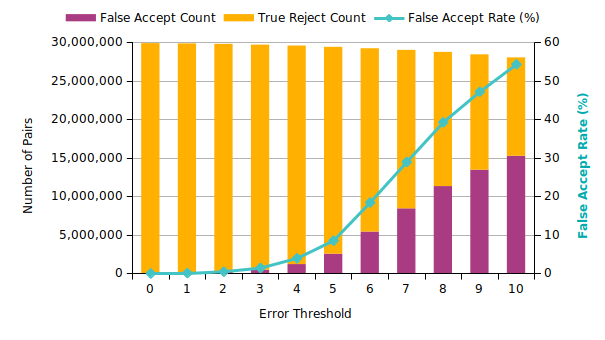
\includegraphics[width=\textwidth]{figures/acc_e5_100bp_stacked.png}
    \caption{False accept analysis - 100bp.}
    \label{fig:acc_e5_100bp_stacked}
  \end{minipage}
\end{figure}

%%%%%%%%%%%%%%%%%%%%%%%%%%%%%%%%%%%%%%%%%%%%%%%%%%%%%%%%

Compared with Edlib's global alignment results, GateKeeper-GPU's false reject count is always $0$ for all data sets, indicating that it never rejects a true extendable read and reference segment pair. For mrFAST's potential mappings, Figure \ref{fig:acc_e5_100bp_stacked} illustrates the number of false accepts and true rejects and the false accept rate as a percentage of the number of false accepts over the number of rejected pairs by Edlib, with respect to the error threshold. The detailed results of these experiments and the figures for the remaining data sets are available in Sup. Material IV.

Considering the results of these experiments, we make the following observations regarding the accuracy of GateKeeper-GPU:~1)~Up to $\sim$3\% error thresholds of all read lengths, GateKeeper-GPU can correctly reject more than $90\%$ of the mappings with less than $10\%$ of false accept ratio and with no false reject.
2)~Even though the efficiency of filtering decreases when the error threshold increases, filtering still continues to serve without a steep drop in efficiency for the largest error threshold allowed~($10\%$). 3)~With increased read length, the false accept rate increment and filtering efficiency decrease become sharper. Furthermore, GateKeeper-GPU can filter out all dissimilar sequence pairs produced by Minimap2 with no false accepts for error threshold \textit{e} = 0~(Sup. Table S.5) and can present a true reject rate of up to 98\% on BWA-MEM's candidate mappings~(Sup. Table S.6).

%%%%%%%%%%%%%%%%%%%%%%%%%%%%%%%%%%%%%%%%%%%%%%%%%%%%%%%%%%
%%%%%%%%%%%%%%%%%%%%%%%%%%%%%%%%%%%%%%%%%%%%%%%%%%%%%%%%%%
\subsubsection{Comparison with Other Pre-alignment Filters}
We compare GateKeeper-GPU's results with five other filtering tools: its original FPGA GateKeeper implementation, SHD, MAGNET, Shouji, and SneakySnake with respect to Edlib's ground truth in the second phase of accuracy analyses. For this purpose, we use low-edit profile~(Set\_1, Sec\_5, and Set\_9) and high-edit profile datasets~(Set\_4, Sec\_8, and Set\_10), previously described in Section 4.1 and presented in Sup. Table S.1 in detail. We perform experiments on these data sets with the filtering error thresholds from $0\%$ to $10\%$ of their corresponding read length.  We retrieved other tools' false accept and reject counts from the Sup. Material of the Shouji manuscript. To maintain a fair comparison in this test series, we include the undefined pairs and mark these pairs as falsely accepted in GateKeeper-GPU's results where necessary.

%%%%%%%%%%%%%%%%%%%%%%%%%%%%%%%%%%%%%%
%100bp
\begin{figure}[!htbp]
  \centering
  \begin{minipage}[b]{0.45\textwidth}
    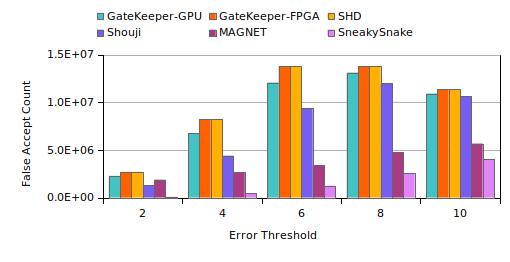
\includegraphics[width=\textwidth]{figures/FP_e2_100bp.png}
    \caption{False accept comparison for Set\_1 with a read length of 100bp and the number of undefined pairs is 28,009.}
    \label{fig:FP_e2_100bp}
  \end{minipage}
\end{figure}
%%%%%%%%%%%%%%%%%%%%%%%%%%%%%%%%%%%%%%

Figure \ref{fig:FP_e2_100bp} and Sup. Figures S.7 to S.11 demonstrate the number of falsely accepted pairs by different tools across the same datasets with varying error thresholds. Even though GateKeeper-GPU has undefined pairs in its false accept count, we see that it has a less false accept rate in most of the cases and can produce up to $52\times$ less number of false accepts~(Table S.10, \textit{e} = 9) when compared to original GateKeeper-FPGA and SHD. We observe that both GateKeeper-FPGA and SHD completely stop filtering in high error thresholds of high-edit profile datasets and accept all pairs~(30 million). In contrast, GateKeeper-GPU still functions in those cases and continues to decrease the number of potential mappings correctly. This suggests that the small modifications made on the GateKeeper algorithm for leading and trailing parts of the bitvectors, explained in detail in Section 3.4, improve the accuracy and help GateKeeper-GPU keep its consistency without completely letting loose filtering in high error thresholds.

In all the tests, SneakySnake and MAGNET have the lowest number of false accepts. However, we notice that MAGNET produces some false accepts for exact matching when the error threshold is 0 as seen in Sup. Figure S.8, and generates false rejects in some cases where GateKeeper-GPU and other filters do not have false rejects. GateKeeper-GPU rarely produces false accepts in the exact matching, and the number of false accepts in these cases is always lower than MAGNET. Finally, for datasets with read lengths 150bp and 250bp, GateKeeper-GPU and Shouji have similar false accept rates, but Shouji's false accept count is less than GateKeeper-GPU. More detailed results of these tests are available in Sup. Material V.

%%%%%%%%%%%%%%%%%%%%%%%%%%%%%%%%%%%%%%%%%%%%%%%%%%%%%%%%%%
%%%%%%%%%%%%%%%%%%%%%%%%%%%%%%%%%%%%%%%%%%%%%%%%%%%%%%%%%%
\subsection{Filtering Throughput Analysis}
To assess GateKeeper-GPU's filtering throughput, we perform experiments on datasets Set\_3, Set\_7, and Set\_11. With respect to kernel time~(i.e., kt) and filter time~(i.e., ft), we calculate the filtering throughput of GateKeeper-GPU. We report the results with filtering error thresholds \{2, 5\}, \{4, 10\}, and  \{6, 10\} for the datasets with read lengths 100bp, 150bp, and 250bp respectively. Table \ref{tab:100bp_filtering_throughput} contains the filtering throughput of GateKeeper-CPU and GateKeeper-GPU with different values for encoding in device and host designs in terms of billions of filtrations in 40 minutes. For GateKeeper-CPU, kernel time represents the time exclusively spent by the function that contains the GateKeeper algorithm. We provide GateKeeper-CPU's results for single-core and 12-core experiments, but we make comparisons based on 12-core results. Please refer to Sup. Material VI for the detailed results of these experiments.

Considering filter time results in Setup\_1, GateKeeper-GPU can filter up to $3\times$ and $20\times$ more pairs than 12-core GateKeeper-CPU, with single and 8 GPUs, respectively (Sup. Table S.15, device\_encoded, 250bp, \textit{e} = 10). In terms of only kernel time, GateKeeper-GPU's filtering throughput can reach up to $72\times$ and $456\times$ more than 12-core GateKeeper-CPU, with single and 8 GPUs, respectively~(Sup. Table S.15, host\_encoded, 250bp, \textit{e} = 6). In Setup\_2 with a single GPU, GateKeeper-GPU can filter up to $2\times$ and $16\times$ more pairs than 12-core GateKeeper-CPU with respect to filter time and kernel time (Sup. Table S.15, device\_encoded, 250bp, \textit{e} = 10).

%%%%%%%%%%%%%%%%%%%%%%%%%%%%%%%%%%%%%%%%%%%%%%%%%%%%%%%%%%%%%%
% 100bp- Geforce&Tesla - Filtering Throughput
\begin{table}[!htbp]
\caption{Filtering throughput for 100bp sequences.}
\label{tab:100bp_filtering_throughput}
\begin{adjustbox}{max width=0.49\textwidth}
\Large
\begin{tabular}{lcc|rr|rr|rr}
                                                        &                                         & \multicolumn{1}{c}{\textbf{} }  & \multicolumn{2}{c}{\textbf{GateKeeper-CPU} }                                    & \multicolumn{2}{c}{\textbf{Device-encoded} }                               & \multicolumn{2}{c}{\textbf{Host-encoded} }                                 \\  
\cline{4-9}   
\multicolumn{1}{c}{}    \rule{0pt}{3ex}                                 &                                         & \multicolumn{1}{c}{\textit{e}~} & \multicolumn{1}{r}{\textit{1-Core } } & \multicolumn{1}{r}{\textit{12-Cores } } & \multicolumn{1}{r}{\textit{1-GPU } } & \multicolumn{1}{r}{\textit{8-GPU} } & \multicolumn{1}{r}{\textit{1-GPU } } & \multicolumn{1}{r}{\textit{8-GPU}}  \\ 
\cline{3-9}
\multirow{4}{*}{Setup\_1}                     &  \rule{0pt}{2ex} \multirow{2}{*}{kt}                     & 2                               & 0.7                                   & 7.2                                     & 244.8                                & 1,189.8                             & 476.8                                & \textbf{3,198.4}                    \\
                                                        &                                         & 5                               & 0.4                                   & 3.9                                     & 150.8                                & 1,041.4                             & 249.3                                & \textbf{1,684.7}                    \\ 
\cline{3-9}
                                                        &  \rule{0pt}{2ex} \multirow{2}{*}{ft}                     & 2                               & 0.6                                   & 6.5                                     & 7.7                                  & \textbf{39.2}                       & 3.0                                  & 14.4                                \\
                                                        &                                         & 5                               & 0.4                                   & 3.7                                     & 7.6                                  & \textbf{37.8}                       & 2.9                                  & 14.2                                \\ 
\cline{2-9}
\multicolumn{1}{r}{\multirow{4}{*}{Setup\_2}}  \rule{0pt}{2ex}& \multicolumn{1}{r}{\multirow{2}{*}{kt}} & 2                               & 0.7                                   & 5.5                                     & 41.1                                 & NA                                  & \textbf{72.2}                        & NA                                  \\
\multicolumn{1}{r}{}                                    & \multicolumn{1}{r}{}                    & 5                               & 0.3                                   & 3.0                                     & 29.1                                 & NA                                  & \textbf{42.0}                        & NA                                  \\ 
\cline{3-9}
\multicolumn{1}{r}{}             \rule{0pt}{2ex}                        & \multicolumn{1}{r}{\multirow{2}{*}{ft}} & 2                               & 0.6                                   & 4.9                                     & \textbf{6.1}                         & NA                                  & 2.7                                  & NA                                  \\
\multicolumn{1}{r}{}                                    & \multicolumn{1}{r}{}                    & 5                               & 0.3                                   & 2.8                                     & \textbf{5.7}                         & NA                                  & 2.7                                  & NA                                  \\
\cline{3-9}
\end{tabular}
\end{adjustbox}
\begin{minipage}{0.49\textwidth}
\vspace*{0.2cm}
\scriptsize
Filtering throughput is calculated wrt. kernel time (kt) and filter time (ft), in terms of billions of pairs in 40 minutes. The highest filtering throughput within the row is in bold font. \textit{e = }error threshold.
\end{minipage}
\end{table}
%%%%%%%%%%%%%%%%%%%%%%%%%%%%%%%%%%%%%%%%%%%%%%%%%%%%%%%%%%%5

Although in some cases, 12-core GateKeeper-CPU exhibits similar performance to single device GateKeeper-GPU with encoding in host option in terms of filter time, the biggest advantage of GPU implementation over CPU implementation is having a constant performance when the error threshold increases. While the filter time remains constant in both device-encoded and host-encoded GateKeeper-GPU, the growth in GateKeeper-CPU’s filter time is almost linear with increasing error threshold. Hence, GateKeeper-GPU performs better with high error thresholds.

GateKeeper-GPU's performance changes depending on the encoding actor~(as host or device) as Figure \ref{fig:thr_encodingfact}, and Sup. Figures S.13 and S.14 show. We notice that encoding in the host leads to higher throughput in all three different sequence lengths when we consider kernel time (depicted by bars in the figures). Especially in lower error thresholds, the difference between host-encoded and device-encoded throughput values is significant. On the other hand, it turns into the opposite situation when filter time (depicted by lines in figures) is considered. From these observations, we conclude that the encoding procedure creates a bottleneck for the workflow of GateKeeper-GPU, and the encoding actor plays a critical role in efficiency. Since GateKeeper-GPU is an intermediate tool, choosing the right encoding actor in different scenarios can lead to the optimum results. 

%\vspace{-2mm}
%%%%%%%%%%%%%%%%%%%%%%%%%%%%%%%%%%%%%%%%%%
%figure: Encoding actor E5
%100bp
\begin{figure}[!htbp]
  \centering
  \begin{minipage}[b]{0.45\textwidth}
    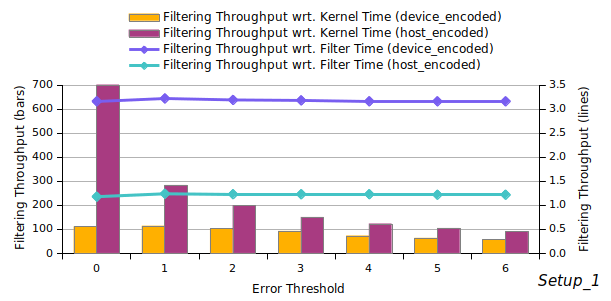
\includegraphics[width=\textwidth]{figures/thr_encodingfact_set1_e5.png}
  \end{minipage}
  %\hfill
  \begin{minipage}[b]{0.46
  \textwidth}
    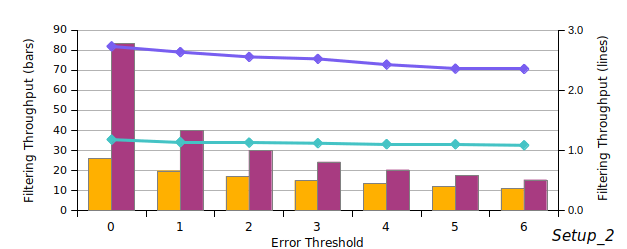
\includegraphics[width=\textwidth]{figures/thr_encodingfact_set2_e5.png}
  \end{minipage}
  \vspace{0.2cm}
  \caption{\scriptsize Effect of the encoding actor~(device or host) on filtering throughput (millions of filtrations per second) of single-GPU GateKeeper-GPU for 100bp reads. Filtering throughput is calculated with respect to kernel time: bars, and filter time: lines.}
  \label{fig:thr_encodingfact}
\end{figure}
%%%%%%%%%%%%%%%%%%%%%%%%%%%%%%%%%%%%%%%%%%%%%%%%%%%%%%%%

We previously stated that the error threshold has a negligible effect on GateKeeper-GPU's performance and can yield a constant efficiency with increasing error threshold. Apart from the encoding actor, the read length is another factor that influences GateKeeper-GPU's filtering throughput. In longer sequences, GateKeeper-GPU tends to filter with a lower throughput rate, as shown in Figure \ref{fig:thr_readlength}. 

%%%%%%%%%%%%%%%%%%%%%%%%%%%%%%%%%%%%%%%%%%%%%%%%%
% Fig: effect of read length
\begin{figure}[!htbp]
\centering
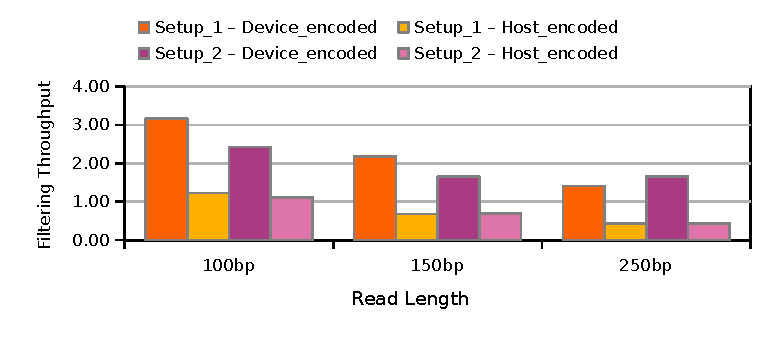
\includegraphics[width=0.45\textwidth]{figures/thr_readlength.pdf}
%\vspace{0.2cm}
\caption{\scriptsize Effect of read length on single-GPU GateKeeper-GPU's filtering throughput (millions of filtrations per second) with error threshold \textit{e} = 4. Filtering throughput is calculated with respect to filter time.}
\label{fig:thr_readlength}
\end{figure}
%%%%%%%%%%%%%%%%%%%%%%%%%%%%%%%%%%%%%%%%%%%%%%%%%%%

To understand how GateKeeper-GPU's performance scales with increasing the number of GPGPU devices, we performed tests with 8 GPUs~(Figure \ref{fig:thr_multigpu} and Sup. Figure S.15). With respect to filter time~(lines in Figure \ref{fig:thr_multigpu}), GateKeeper-GPU with encoding in the device experiences a steeper performance increase as the number of devices increases. On the other hand, regarding the kernel time~(bars in Figure \ref{fig:thr_multigpu}), encoding in the device makes GateKeeper-GPU show a slower performance growth with more devices when compared to encoding in the host. Considering the kernel time, adding one more device to the system almost doubles GateKeeper-GPU's throughput in some cases when encoding is done in the host. Therefore, GateKeeper-GPU is better adapted to a multi-GPU environment in a host-encoded fashion. 

%%%%%%%%%%%%%%%%%%%%%%%%%%%%%%%%%%%%%%%%%%%%%%%%%
%figure: multigpu
\begin{figure}[!htbp]
\centering
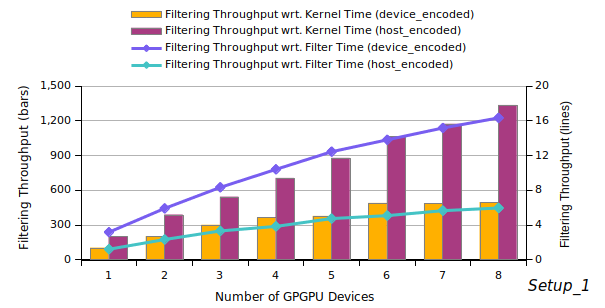
\includegraphics[width=0.45\textwidth]{figures/thr_multigpu_setting1_e5.png}
%\vspace{1mm}
\caption{\scriptsize Multi-GPU filtering throughput~(millions of filtrations per second) of GateKeeper-GPU in Setup\_1 100bp reads with error threshold \textit{e} = 2. Filtering throughput is calculated with respect to kernel time: bars, and filter time: lines.}
\label{fig:thr_multigpu}
\end{figure}

%%%%%%%%%%%%%%%%%%%%%%%%%%%%%%%%%%%%%%%%%%%%%%%%%%%%%%%

In general, GateKeeper-GPU's throughput is lower in Setup\_2 than in Setup\_1 using a single GPU. Setup\_2 does not support data prefetching and has a smaller global memory, both of which are crucial for GateKeeper-GPU's performance, therefore it tends to produce fewer filtrations than Setup\_1.

Due to platform differences, we believe it would not be completely fair to make a comparison between GateKeeper-GPU and other filtering tools in terms of filtering throughput. To create a point of reference, we can briefly express the following observations. Within 40 minutes, GateKeeper-FPGA and SHD can filter up to $\sim$4 trillion and $86$ billion potential mappings, respectively. Regarding kernel time, GateKeeper-GPU can filter more than 7 trillion pairs with 8-GPUs in host-encoding fashion, in Setup\_1 on sequence length 100bp with error threshold 0. However, when considering filter time, the highest number of filtration pairs is $\sim$40 billion, on the same dataset conditions with a device-encoding option on 8 GPUs. 

Considering all of the observations on the filtering throughput of GateKeeper-GPU, we conclude that when the other variables are kept constant, read length and encoding actor (host or device) are critical variables that directly affect the performance, whereas error threshold has a negligible effect. Data prefetching also plays an important role as a platform-dependent factor.   

\subsection{Whole Genome Accuracy \& Performance Analysis}
We evaluate the accuracy and performance of GateKeeper-GPU in full read mapping workflow using four real and two simulated data sets~(Sup. Table S.1).
%%%%%%%%%%%%%%%%%%%%%%%%%%%%%%%%%%%%%%%%%%%%%%%%%%%%%%%%%%%5%%
% Whole genome accuracy table  100bp

\begin{table}[!htbp]
\caption{Whole genome mapping information with pre-alignment filtering on real dataset}
\label{tab:whole_gen}
\begin{adjustbox}{max width=0.49\textwidth}
\begin{tabular}{rr|r|r|r|r}
\multicolumn{1}{r}{\textit{mrFAST w/} } & \multicolumn{1}{r}{\textit{-e }} & \multicolumn{1}{r}{\textit{Mappings} } & \multicolumn{1}{r}{\textit{Mapped Reads }} & \multicolumn{1}{r}{\textit{Verification Pairs }} & \multicolumn{1}{c}{\textit{Rejected Pairs (Reduction) }}  \\ 
\hline
\multirow{2}{*}{No Filter}       \rule{0pt}{2ex}        & 0                               & 13,800,412                             & 3,052,036                                  & 257,927,779                                      & NA                                                        \\
                                        & 5                               & 639,841,922                            & 3,887,943                                  & 45,664,847,515                                   & NA                                                        \\ 
\hline
\multirow{2}{*}{GateKeeper-GPU}    \rule{0pt}{2ex}      & 0                               & 13,800,412                             & 3,052,036                                  & 13,824,296                                       & 244,103,483 ( 94 \% )                                     \\
                                        & 5                               & 639,820,825                            & 3,887,939                                  & 4,289,442,302                                    & 41,375,405,213 ( 90 \% )                                  \\
\hline
\end{tabular}
\end{adjustbox}
\begin{minipage}{0.49\textwidth}
\vspace*{0.2cm}
\scriptsize
Mapping information by running mrFAST on ERR240727\_1~(100bp) data set with error thresholds e = 0 and e = 5. The entries represent the number of the corresponding metrics. \textit{-e}: mrFAST's edit distance threshold and error threshold for filtering.
\end{minipage}
\end{table}
%%%%%%%%%%%%%%%%%%%%%%%%%%%%%%%%%%%%%%%%%%%%%%%%%%%%%%%%%%%%%%%

For the accuracy tests, we carry out experiments with error thresholds \textit{e} = 0 and \textit{e} = 5 on ERR240727\_1; with error thresholds \textit{e} = 15 for sim\_set\_1 and \textit{e} = 8 for sim\_set\_2. Table \ref{tab:whole_gen}, Sup. Tables  S.24 to S.26 contain mapping information of mrFAST with GateKeeper-GPU. We observe that GateKeeper-GPU successfully filters out faulty mappings and reduces the number of potential mappings correctly by 94\% and 90\% for \textit{e} = 0 and \textit{e} = 5, respectively. We notice a small discrepancy between the total number of mappings and mapped reads produced by mrFAST with and without GateKeeper-GPU when \textit{e} = 5 on the real dataset, as shown in Table \ref{tab:whole_gen}. To analyze these potential false rejects more deeply, we collected some information about the candidate pairs that GateKeeper-GPU rejected and the verification accepted with random sampling. We ran Edlib's global alignment on these samples and found that all these pairs exceeded the error threshold, supporting GateKeeper-GPU's decision to reject. Furthermore, we never experience false rejects in our deep accuracy analysis, as explained in Section 5.1. Therefore, GateKeeper-GPU can \textit{increase} the accuracy of the alignment of mrFAST by rejecting these mappings.

%%%%%%%%%%%%%%%%%%%%%%%%%%%%%%%%%%%%%%%%%%%%%%%%%%%%%%
% Theoretical Values Table for edit 5
\begin{table}[!htbp]
\caption{Theoretical speedup vs. achieved speedup in verification.}
\label{tab:theoreticalvsachieved}
\begin{adjustbox}{max width=0.49\textwidth}
\begin{tabular}{r|rr|rr}
\multicolumn{1}{r}{}                     & \multicolumn{2}{c}{\textbf{Theoretical DP Time / Speedup} }                     & \multicolumn{2}{c}{\textbf{Achieved DP Time / Speedup} }  \\
\multicolumn{1}{r}{ \textit{mrFAST w/} } & \textit{Setup\_1}                      & \multicolumn{1}{r}{\textit{Setup\_2} } & \textit{Setup\_1}    & \textit{Setup\_2}                  \\ 
\hline  \rule{0pt}{2ex}
No Filter                                & NA                                     & NA                                     & 3.99h                & 4.66h                              \\ 
\hline  \rule{0pt}{2ex}
GateKeeper-GPU (d)                       & \multirow{2}{*}{0.37h / 10.6$\times$ } & \multirow{2}{*}{0.44h / 10.6$\times$ } & 1.08h / 3.7$\times$  & 1.22h / 3.8$\times$                \\
GateKeeper-GPU (h)                       &                                        &                                        & 1.10h / 3.6$\times$  & 1.24h / 3.7$\times$                \\
\hline
\end{tabular}
\end{adjustbox}
\begin{minipage}{0.49\textwidth}
\vspace*{0.2cm}
\scriptsize
Calculations and measurements represent the values for running mrFAST with single-GPU GateKeeper-GPU (encoding in d: device, h: host) on 100bp data set with error threshold \textit{e} = 5. GateKeeper-GPU provides a 90\% reduction in the number of potential mappings. DP: dynamic programming based verification.
\end{minipage}
\end{table}
%%%%%%%%%%%%%%%%%%%%%%%%%%%%%%%%%%%%%%%%%%%%%%%%%%%%%%%

With respect to the amount of reduction GateKeeper-GPU provides in the number of candidate mappings that enter the verification stage, we calculate the theoretical verification time and speedup by direct proportion. Table \ref{tab:theoreticalvsachieved} compares the theoretical and achieved speedup for the verification stage with GateKeeper-GPU on 100bp data set with \textit{e} = 5. Based on our calculations, we expect a $10.6\times$ speedup on verification, and in practice, verification can achieve up to $3.8\times$ speedup. 

For evaluating how much impact the reduction in the number of candidate mappings that enter verification has on whole genome alignment speedup on a large scale, we construct Table \ref{tab:wholegenspeedup}, Sup. Tables S.24 and S.25. We sum up the time spent on the filtering and verification compared to the verification time of mrFAST when no pre-alignment filtering is used. For filtering time, we consider the kernel time for GateKeeper-GPU. We report only the speedup values of GateKeeper-FPGA since it requires a different platform and the time measurements cannot be scaled for our setting. GateKeeper-GPU has better accuracy than GateKeeper-FPGA and can filter out more candidate mappings while GateKeeper-FPGA performs better than GateKeeper-GPU in terms of accelerating the whole alignment process.

%%%%%%%%%%%%%%%%%%%%%%%%%%%%%%%%%%%%%%%%%%%%%%%%%%%%%%%
% Speed-up Comparison Table (100bp - edit 5)
\begin{table}[!htbp]
\caption{Speedup comparison of mrFAST with different pre-alignment filters on a real dataset.}
\label{tab:wholegenspeedup}
\begin{adjustbox}{max width=0.49\textwidth}
\Large
\begin{tabular}{r|ll|ll}
\multicolumn{1}{c}{} & \multicolumn{2}{c}{\textbf{Filtering + DP Time / Speedup} }   & \multicolumn{2}{c}{\textbf{Overall Time / Speedup} }  \\
\rule{0pt}{3ex}
 \textit{mrFAST w/}  & \textit{Setup\_1}    & \multicolumn{1}{l}{\textit{Setup\_2} } & \textit{Setup\_1}    & \textit{Setup\_2}              \\ 
\hline \rule{0pt}{2ex}
No Filter            & 3.99h / NA            & 4.66h / NA                             & 6.85h / NA           & 7.81h / NA                     \\
GateKeeper-GPU (d)   & 1.38h / 2.9$\times$  & 2.85h / 1.6$\times$                    & 4.79h / 1.4$\times$  & 6.63h / 1.2$\times$            \\
GateKeeper-GPU (h)   & 1.38h / 2.9$\times$  & 2.77h / 1.7$\times$                    & 5.26h / 1.3$\times$  & 6.82h / 1.2$\times$            \\
GateKeeper-FPGA      & \multicolumn{2}{c|}{*41$\times$ }                             & \multicolumn{2}{c}{*9.7$\times$ }                     \\
\hline
\end{tabular}
\end{adjustbox}
\begin{minipage}{0.49\textwidth}
\vspace*{0.2cm}
\scriptsize
Speedup comparison between mrFAST's performance with GateKeeper-GPU with single GPU~(encoding in d: device, h: host) and GateKeeper-FPGA on ERR240727\_1~(100bp) data set with error threshold \textit{e} = 5. DP: verification. *values were retrieved from GateKeeper's manuscript~\cite{Alser2017}.
\end{minipage}
\end{table}
% %%%%%%%%%%%%%%%%%%%%%%%%%%%%%%%%%%%%%%%%%%%%%%%%%%%%%%

For 100bp reads, GateKeeper-GPU can accelerate the verification stage up to $2.9\times$ and $1.7\times$ with Setup\_1 and Setup\_2 when filtering and verification are combined. We directly observe the benefit of data prefetching on Setup\_1 since it creates a larger speedup when compared to Setup\_2. These speedup values reflect on the overall speedup as up to $1.4\times$ and $1.2\times$, respectively.

Even though GateKeeper-GPU can correctly discard $97\%$ of candidate mappings~(Sup. Table S.24), we notice that the kernel time is longer for 300bp and additional operations, such as preparing buffers and data transfer, which are inserted into mrFAST's workflow and required by pre-alignment filtering with GPU, dominate over the time gained from sequence alignment. Also, the data set size is small. Because GateKeeper-GPU exhibits a better performance with large batch sizes, the size of the dataset can be another factor for the absence of speedup. On the 150bp simulated dataset, GateKeeper-GPU can achieve speedup for both verification and overall time in Setup\_1~(Sup. Table S.25). Setup\_2 is deprived of data prefetching and has a smaller global memory, thus the acceleration on verification is not sufficient to reflect the impact on overall mapping duration. These different results of the two device setups validate the effect of data prefetching and global memory size on unified memory usage.  

%%%%%%%%%%%%%%%%%%%%%%%%%%%%%%%%%%%%%%%%%%%%%%%%%%%%%%%%%
%%%%%%%%%%%%%%%%%%%%%%%%%%%%%%%%%%%%%%%%%%%%%%%%%%%5%%%%
\subsection{Resource Utilization and Power Analysis}

\subsubsection{Resource Utilization}
The smallest number of registers that the GateKeeper-GPU kernel uses to complete its functionalities fully is 40 registers. The register count can increase to 48 registers per thread in different cases. The maximum theoretical occupancy that can be reached with 48 registers per thread is $63\%$, but the number of threads per block should be at most 256, a quarter of the maximum number of threads per block. Using fewer threads decreases the batch size for a single transfer between host and device, eventually increasing the number of transfers. In our experience, the majority of the time is spent on preprocessing rather than on the kernel. Hence, having the smallest number of transfers is optimal in our scenario, and we opt to set the maximum number of threads for maximized batch size. 

Following this logic, GateKeeper-GPU's theoretical warp occupancy is $50\%$.  In Setup\_1 with encoding in device option, the average achieved occupancy is $48.5\%$ and $49.2\%$ for 100bp and 250bp sequence sets, respectively. When the sequences are encoded in the host, the average occupancy becomes $47.5\%$ and $48.9\%$. Likewise, in Setup\_2 with encoding in the device option, the average achieved occupancy is $46.8\%$ and $48.7\%$ for 100bp and 250bp sequence sets. When sequences are encoded in the host, the average occupancy becomes $44.6\%$ and $47.8\%$, respectively. 

GateKeeper-GPU's achieved occupancy is very close to theoretical warp occupancy. This shows that the warp scheduler can issue new instructions with negligible or no stalls, and the theoretical number of warps is almost reached while SM is active. Therefore, within this limit of register count, the workload within and between the blocks is balanced. On the other hand, because the occupancy is half of its maximum value, average warp execution efficiency is $79.1\%$ and $74.5\%$ in Setup\_1; $80.2\%$ and $76\%$ in Setup\_2 for the 100bp dataset with encoding on device and host, respectively. For the 250bp data set in both device setups, warp execution efficiency is always above $98\%$ on average. This difference created by increasing read length can indicate that occupancy is already at the optimum level for hiding latency in longer sequences.  

GateKeeper-GPU's priority is the effective and full utilization of computing resources to achieve the highest throughput possible. SM efficiency is always above $98\%$ on average and never below $95\%$ regardless of the read length and the encoding actor in both device setups. This high multiprocessor activity shows that the SM(s) are almost never idle during execution. 
%%%%%%%%%%%%%%%%%%%%%%%%%%%%%%%%%%%%%%%%%%%%%%%%%%%%%%%
%%%%%%%%%%%%%%%%%%%%%%%%%%%%%%%%%%%%%%%%%%%%%%%%%%%%%%%
\subsubsection{Power Consumption Analysis}
The power consumption of a single GPGPU device for running GateKeeper-GPU is shown in Table \ref{tab:power} and Sup. Table S.27. For 100bp and 250bp datasets, we run with error thresholds 4 and 10, respectively, to evaluate the average energy use of the kernel. The first observation is the negligible effect of the encoding actor on the kernel power consumption when the read length is 100bp. Results show that encoding the sequences on a device or host does not create a huge difference. Even though encoding in the device puts more workload on the device, the energy consumption is almost the same on average for 100bp reads in Setup\_1  owing to effective parallelism~(Table 6). In general, what creates a difference in power consumption is the increase in the read length. The kernel tends to use more power in longer sequences due to increased memory usage and, eventually, more word processing.


%%%%%%%%%%%%%%%%%%%%%%%% Power Table for Geforce
\begin{table}[!htbp]
\centering
\caption{Power consumption of GateKeeper-GPU in Setup\_1.}
\label{tab:power}
\begin{adjustbox}{max width=0.49\textwidth}
\begin{tabular}{r|rr|rr}
\multicolumn{1}{c}{}                     & \multicolumn{2}{c}{\textbf{Device-encoded} } & \multicolumn{2}{c}{\textbf{Host-encoded} }  \\
\multicolumn{1}{r}{\textit{Power (mW) }} & \textit{100bp}  & \textit{250bp}             & \textit{100bp}  & \textit{250bp}            \\ 
\hline \rule{0pt}{2ex}
min                                      & 8,901           & 8,702                      & 8,803           & 8,628                     \\
max                                      & 113,218         & 238,701                    & 157,730         & 260,681                   \\
average                                  & 61,868          & 89,023                     & 61,881          & 77,109                    \\
\hline
\end{tabular}
\end{adjustbox}
\begin{minipage}{0.49\textwidth}
\vspace*{0.2cm}
\scriptsize
Power Consumption~(milliwatt) for single GPU in Setup\_1. The values were obtained by running the CUDA command-line profiler nvprof. 
\end{minipage}
\end{table}